\documentclass[10pt, oneside]{article} 
\usepackage{amsmath, amsthm, amssymb, calrsfs, wasysym, verbatim, bbm, color, graphics, geometry}
\usepackage{polski}
\usepackage[utf8]{inputenc}
\usepackage[cache=false]{minted}
\usepackage{algorithm}
\usepackage{algorithmicx}
\usepackage[noend]{algpseudocode}
\usepackage{url}
\usepackage{tikz}
\usepackage{pgfplots}
\usepackage{booktabs}
\usepackage[T1]{fontenc}
\usepackage{multirow}

\setminted{linenos=true}

\usetikzlibrary{matrix,arrows,automata}

\geometry{tmargin=.75in, bmargin=.75in, lmargin=.75in, rmargin = .75in}  

\theoremstyle{remark}
\newtheorem*{example}{Przykład}


% Cormen's cost analysis
\newcommand{\TITLE}[1]{\item[#1]}
\renewcommand{\algorithmiccomment}[1]{$/\!/$ \parbox[t]{4.5cm}{\raggedright #1}}
% ugly hack for for/while
\newbox\fixbox
\renewcommand{\algorithmicdo}{\setbox\fixbox\hbox{\ {} }\hskip-\wd\fixbox}
% end of hack
\newcommand{\algcost}[2]{\strut\hfill\makebox[1.5cm][l]{#1}\makebox[4cm][l]{#2}}



\title{MST oraz algorytm Dijktry}
\author{mgr. inż Dominik Filipiak}
%\date{Rok akademicki 2019/2020}

\begin{document}

\maketitle
%\tableofcontents

%\vspace{.25in}
\noindent
\emph{Opracowano na podstawie: Cormen et al., Wprowadzenie do algorytmów}
\section{Minimalne drzewo rozpinające}
Problem minimalnego drzewa rozpinającego to problem znalezienia takiego zbioru $T \subseteq E$, dla którego $w(T) = \sum_{(u,v) \in T} w(u,v)$ jest najmniejsze (gdzie $w(u,v)$ to waga krawędzi między $u$ i $v$).
Przykład: położenie kabla pod systemem drogowym.

\paragraph{Algorytm Kruskala.}
Algorytm zachłanny -- w każdym kroku dodajemy krawędź o najmniejszej wadze.

\begin{algorithm}
    \caption{Algorytm Kruskala}
    \label{alg:mst_kruskal}
    \begin{algorithmic}[1] % The number tells where the line numbering should start
        \Function{MST-Kruskal}{$G, w$} \algcost{}{//$O(|E|\log |V|)$}
			\State $A \gets \varnothing$
        		\For{ \textbf{each} $v \in G.V$}
            		\State $\Call{Make-Set}{v}$ \algcost{}{// jednoelementowe drzewa}
            	\EndFor         
            	\State posortuj niemalejąco $G.E$ względem wag $w$
            	\For{ \textbf{each} $(u, v) \in G.E$ w kolejności niemalejących wag}
            		\If{$\Call{Find-Set}{u} \neq \Call{Find-Set}{v}$}
            		    \State $A \gets A \cup \{(u, v)\}$
            			\State $\Call{Union}{u, v}$
            		\EndIf
            	\EndFor
        \EndFunction
    \end{algorithmic}
\end{algorithm}

\paragraph{Algorytm Prima.}
Również algorytm zachłanny.
\begin{algorithm}[htpb]
    \caption{Algorytm Prima}
    \label{alg:mst_prim}
    \begin{algorithmic}[1] % The number tells where the line numbering should start
        \Function{MST-Prim}{$G, w, r$} \algcost{}{// $O(|E|\log |V|)$}
        		\For{\textbf{each} $u \in G.V$}
        			\State $u.key \gets \infty$
        			\State $u.\pi \gets$ \texttt{NIL}
            	\EndFor         
            	\State $r.key \gets 0$
            \State $Q \gets G.V$
            	\While{ $Q \neq \varnothing$}
            		\State $u \gets \Call{Extract-Min}{Q}$
            		\For{\textbf{each} $v \in G.Adj[u]$}
            			\If{$v \in Q \land w(u,v) < v.key$}
            				\State $v.\pi = u$
            				\State $v.key = w(u,v)$
            			\EndIf
            		\EndFor
            	\EndWhile
        \EndFunction
    \end{algorithmic}
\end{algorithm}

%\begin{figure}[htpb]
%	\centering
%	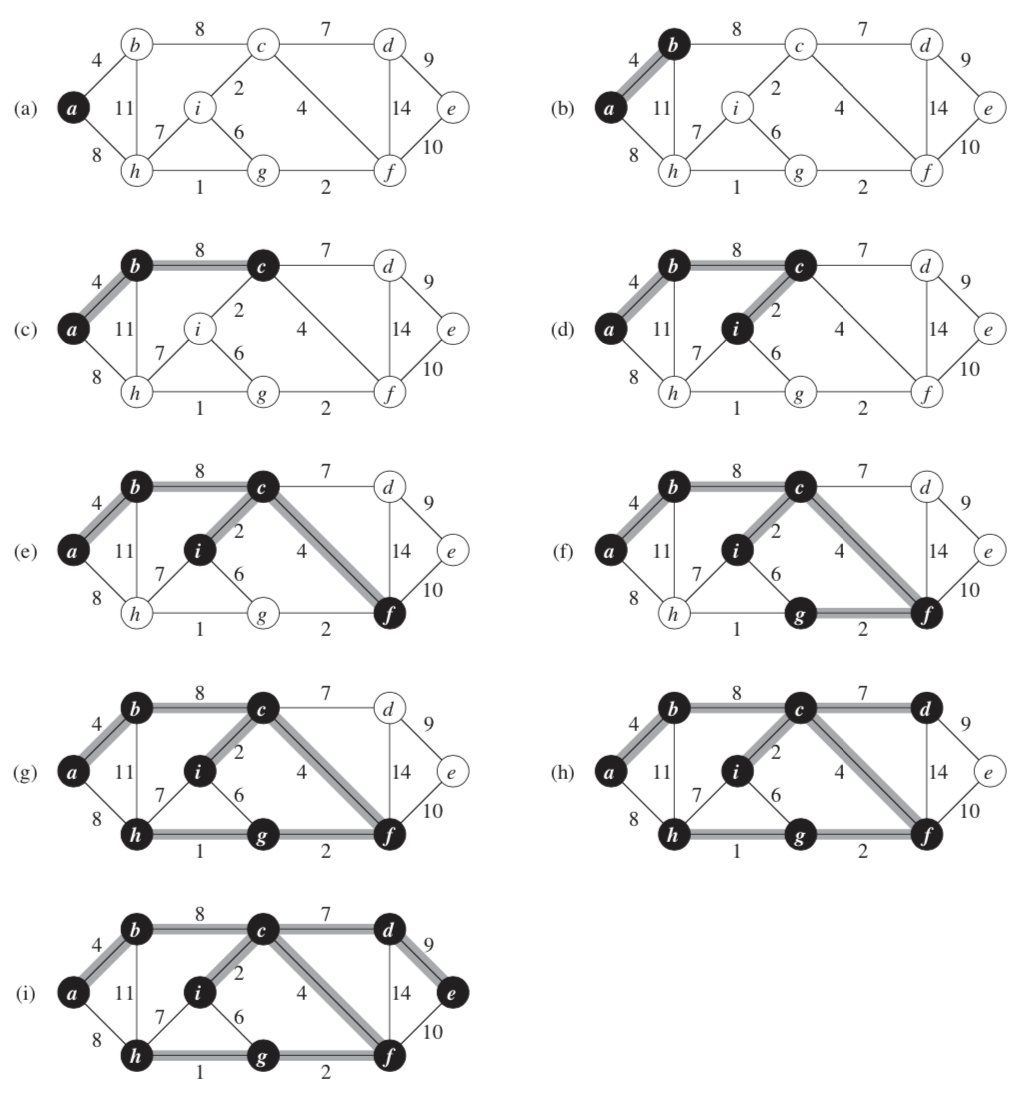
\includegraphics[width=.9\textwidth]{figures/prim}
%	\caption{Algorytm Prima. Źródło: Cormen et al.}
%\end{figure}

\section{Algorytm Dijkstry}
Algorytm Dijkstry służy do rozwiązywania problemu najkrótszych ścieżek z jednym źródłem w ważonym grafie skierowanym z nieujemnymi wagami.
\begin{algorithm}
    \caption{Algorytm Dijkstry}
    \label{alg:dijkstra}
    \begin{algorithmic}[1] % The number tells where the line numbering should start
        \Function{Initialize-Single-Source}{$G, s$} \algcost{}{// $\Theta(|V|)$}
        		\For{ \textbf{each} $v \in G.V$}
            		\State $v.d \gets \infty$
            		\State $v.\pi \gets$ \texttt{NIL} 
            	\EndFor
            	\State $s.d \gets 0$
        \EndFunction
        \Function{Relax}{$u, v, w$} \algcost{}{// $\Theta(1)$}
        		\If{ $v.d > u.d + w(u,v)$}
            		\State $v.d \gets u.d + w(u, v)$
            		\State $v.\pi \gets u$ 
            	\EndIf
        \EndFunction
        \Function{Dijkstra}{$G, u$}            	\algcost{}{// naiwnie $O(|V|^2)$,}
        		\State $\Call{Initialize-Single-Source}{G, s}$ \algcost{}{// da się zejść do $O(|V|\log |V| + |E|)$}
        		\State $S \gets \varnothing$ \algcost{}{// ale wymaga to kopca Fibonacciego}
            	\State $Q \gets G.V$
            \While{$Q \neq \varnothing$}
        			\State $u \gets \Call{Extract-Min}{Q}$
        			\State $S \gets S \cup \{u\}$
        			\For{\textbf{each} $v \in G.Adj[u]$}
        				\State $\Call{Relax}{u, v, w}$
        			\EndFor
            	\EndWhile
        \EndFunction
    \end{algorithmic}
\end{algorithm}

%\begin{figure}[htpb]
%	\centering
%	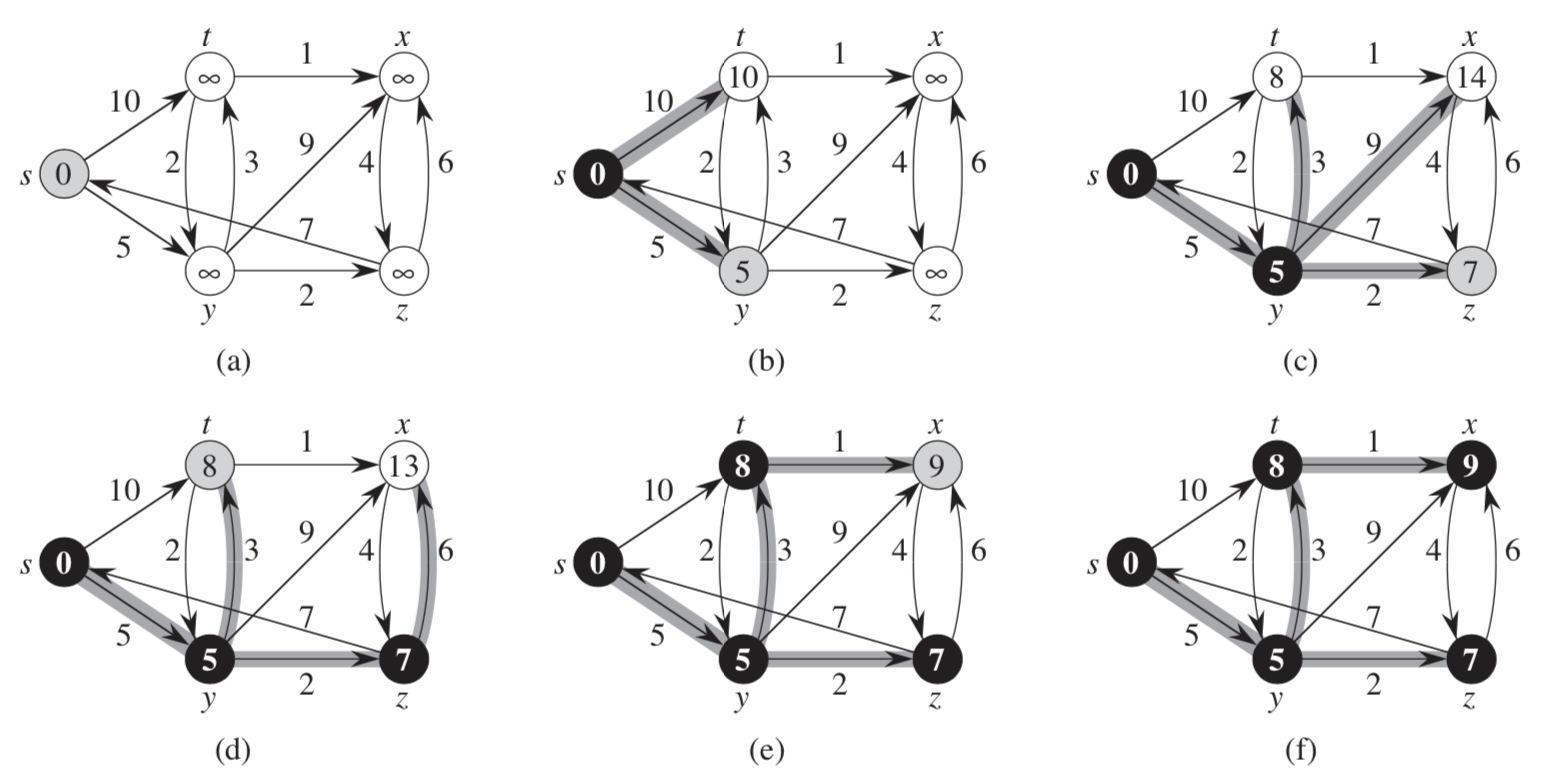
\includegraphics[width=.9\textwidth]{figures/dijkstra}
%	\caption{Algorytm Dijkstry. Źródło: Cormen et al.}
%\end{figure}
%
%\section{Wyszukiwanie wzorca w tekście}
%
%\subsection{Wyszukiwanie naiwne}
%
%\subsection{Algorytm Aho-Corasik}
%
%\section{NP-zupełność. Czy P=NP?}
\end{document}